\section{Reactor Cavity Cooling System}\label{Section:RCCS}
The primary motivation behind this stability work is the so-called \Acronym{RCCS}, which is a safety system for certain proposed Generation IV reactor designs.
A definition and discussion of this safety system for full-scale application is discussed first and followed by a description of an experimental test facility at the \TheUniversity.

\subsection{Full-Scale System}
The \Acronym{NGNP} is a thermal-spectrum, gas-cooled reactor designed to be able to produce electricity as well as process heat for industrial applications.
A novel feature of the \Acronym{NGNP} is the \Acronym{RCCS}.
The \Acronym{RCCS} is a natural circulation system of ducts designed as the \Acronym{NGNP}'s ultimate heat sink for decay heat under a number of accident scenarios.
There are two main designs under consideration which vary mostly in their working fluid: air-cooled and water-cooled.
This work will focus on the water-cooled \Acronym{RCCS} design, leaving air-cooled discussions left to the literature \cite{bechtelnationalinc._450_1993,generalatomics_gas_1996}.


\begin{figure}%
\centering
    \caption[ANL/UW-Madison water-cooled RCCS diagram]{   ANL/UW-Madison  water-cooled RCCS diagram.  
                Water flows from a tank, through the cold leg (blue), through the reactor cavity system, and through the hot leg (red) to some tank on the train at the same conditions (a closed circuit).}%
    \label{Figure:RCCSTotalSystem}%
    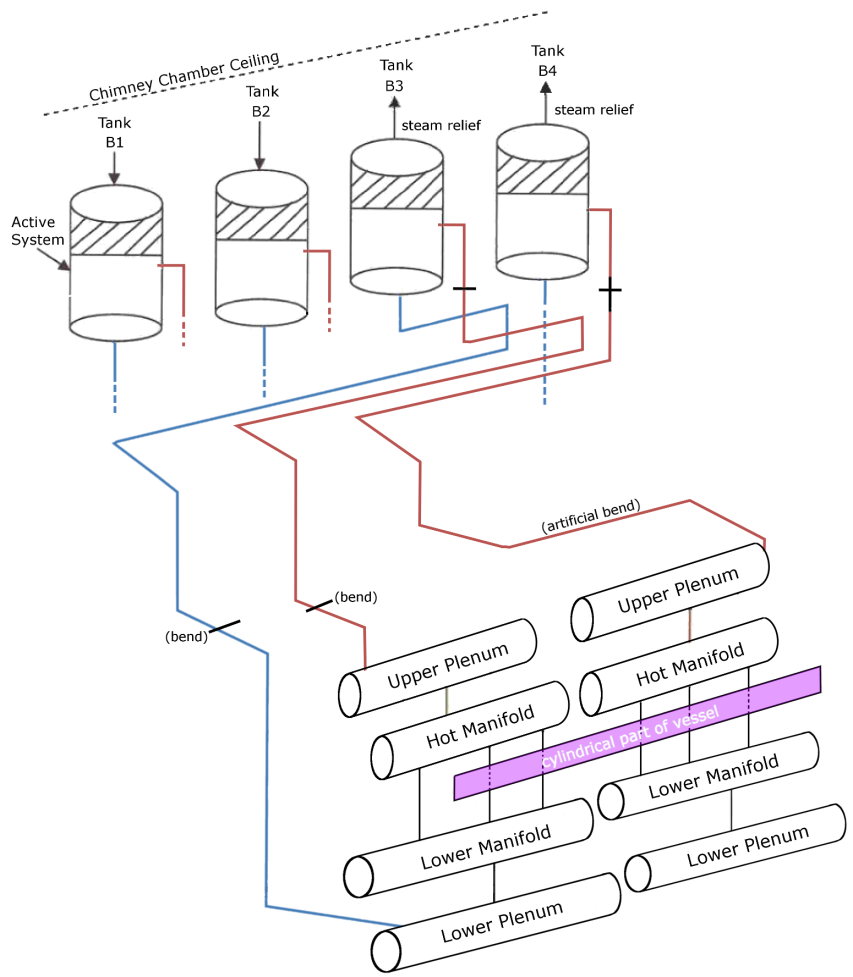
\includegraphics[scale=1.2]{RCCSTotalSystem.png}%
\end{figure}


A collaboration between \Acronym{ANL} and the \TheUniversity\ produced a base, full-scale \Acronym{RCCS} system consisting of a two independent piping networks with each network having four main lines/tanks.
\Cref{Figure:RCCSTotalSystem} outlines the basic design of system B but precludes any detail near the reactor.
The elevation change of the system is on the order of several tens of meters with the reactor cavity portion being approximately twenty meters on its own.
Within the reactor cavity, the eight cold lines of the \Acronym{RCCS} splits into approximately 200 so-called riser pipes that line the cavity wall and ensconce the reactor (see \cref{Figure:RCCSMockup}).
The riser pipes then receive heat from the uninsulated reactor pressure vessel via convection and radiation.
Due to the heating, the fluid that fills the pipes is subjected to a buoyancy force that results in upward flow.

During steady-state operation of the reactor, there is a persistent, parasitic heat loss from the reactor vessel to the \Acronym{RCCS} of approximately $700$ kW.
If the reactor undergoes a loss-of-forced-flow accident with SCRAM, there is an expected peak decay heat load of $1.5$ MW on the \Acronym{RCCS}.
If there is no loss of onsite or offsite power, the \Acronym{RCCS} water storage tanks will be actively cooled, and the system is expected to maintain safe fuel temperatures for the duration of the accident.
In the event of loss of onsite and offsite power (so-called station blackout), the \Acronym{RCCS} can still continue to cool the reactor since the flow is naturally circulating, which is very important for the overall safety of the plant \cite[\SS{50.63}]{nuclearregulatorycomminission_us_2007}.

\begin{figure}%
\centering
    \caption[RCCS near-reactor-riser system]{   Cutaway picture of reactor vessel, RCCS ducts/pipes in the reactor cavity.  
                The low temperature fluid is in blue and the high temperaure fluid is in red.  
                The transparent boxes indicate network encasings. 
                Credit: Darius Lisowski, \TheUniversity.}%
    \label{Figure:RCCSMockup}%
    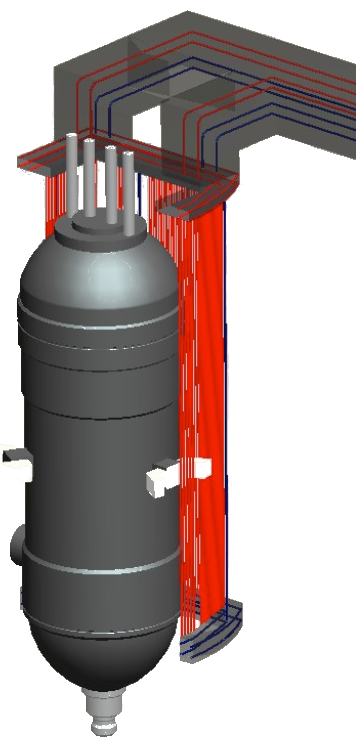
\includegraphics[scale=0.73]{RCCSMockup.png}%
\end{figure}

However, without forced cooling, the reference temperature of the entire water system will continue to rise with continued decay heat exposure.
At some point during the transient, the water leaving the riser system will reach the saturation temperature at atmospheric pressure.  
Due to the gravitational head of all the water on top of the risers, the water will not immediately boil.
Rather, as the water flows to the top of the system, it will instantly boil as it passes into a region where the local pressure falls below the saturation pressure; a process called \textit{flashing}.
This sudden discontinuous jump in substance properties results in flow oscillations because the steam produced from the flash is approximately 1,000 times less dense than the liquid state on the cold side of the system.

\Cref{Figure:RCCSFullScaleMassFlowRate} shows a numerical simulation of the full-scale system.
Before flashing, the mass flow rate is non-oscillatory and increasing due to persistent heating with no cooling.
At the onset of flashing, the flow rate rapidly oscillates and evolves in a complicated manner.
At some point in the evolution, the system's flow rate stabilizes and evolves just as the single phase system.
The period, amplitude, and overall time evolution of these oscillations is subject to numerous factors and various linear and nonlinear effects.
The oscillations are commonly referred to as density wave instabilities since they are driven by the density of the system \cite{achard_analysis_1985}.
These incessant perturbations could potentially lead to large, erratic flow excursions that could pose a safety risk via extreme mechanical or thermal damage.

\begin{figure}%
    \centering
    \caption[RCCS mass flow rate under blackout conditions]{RCCS mass flow rate versus time under blackout conditions.}%
    \label{Figure:RCCSFullScaleMassFlowRate}%
    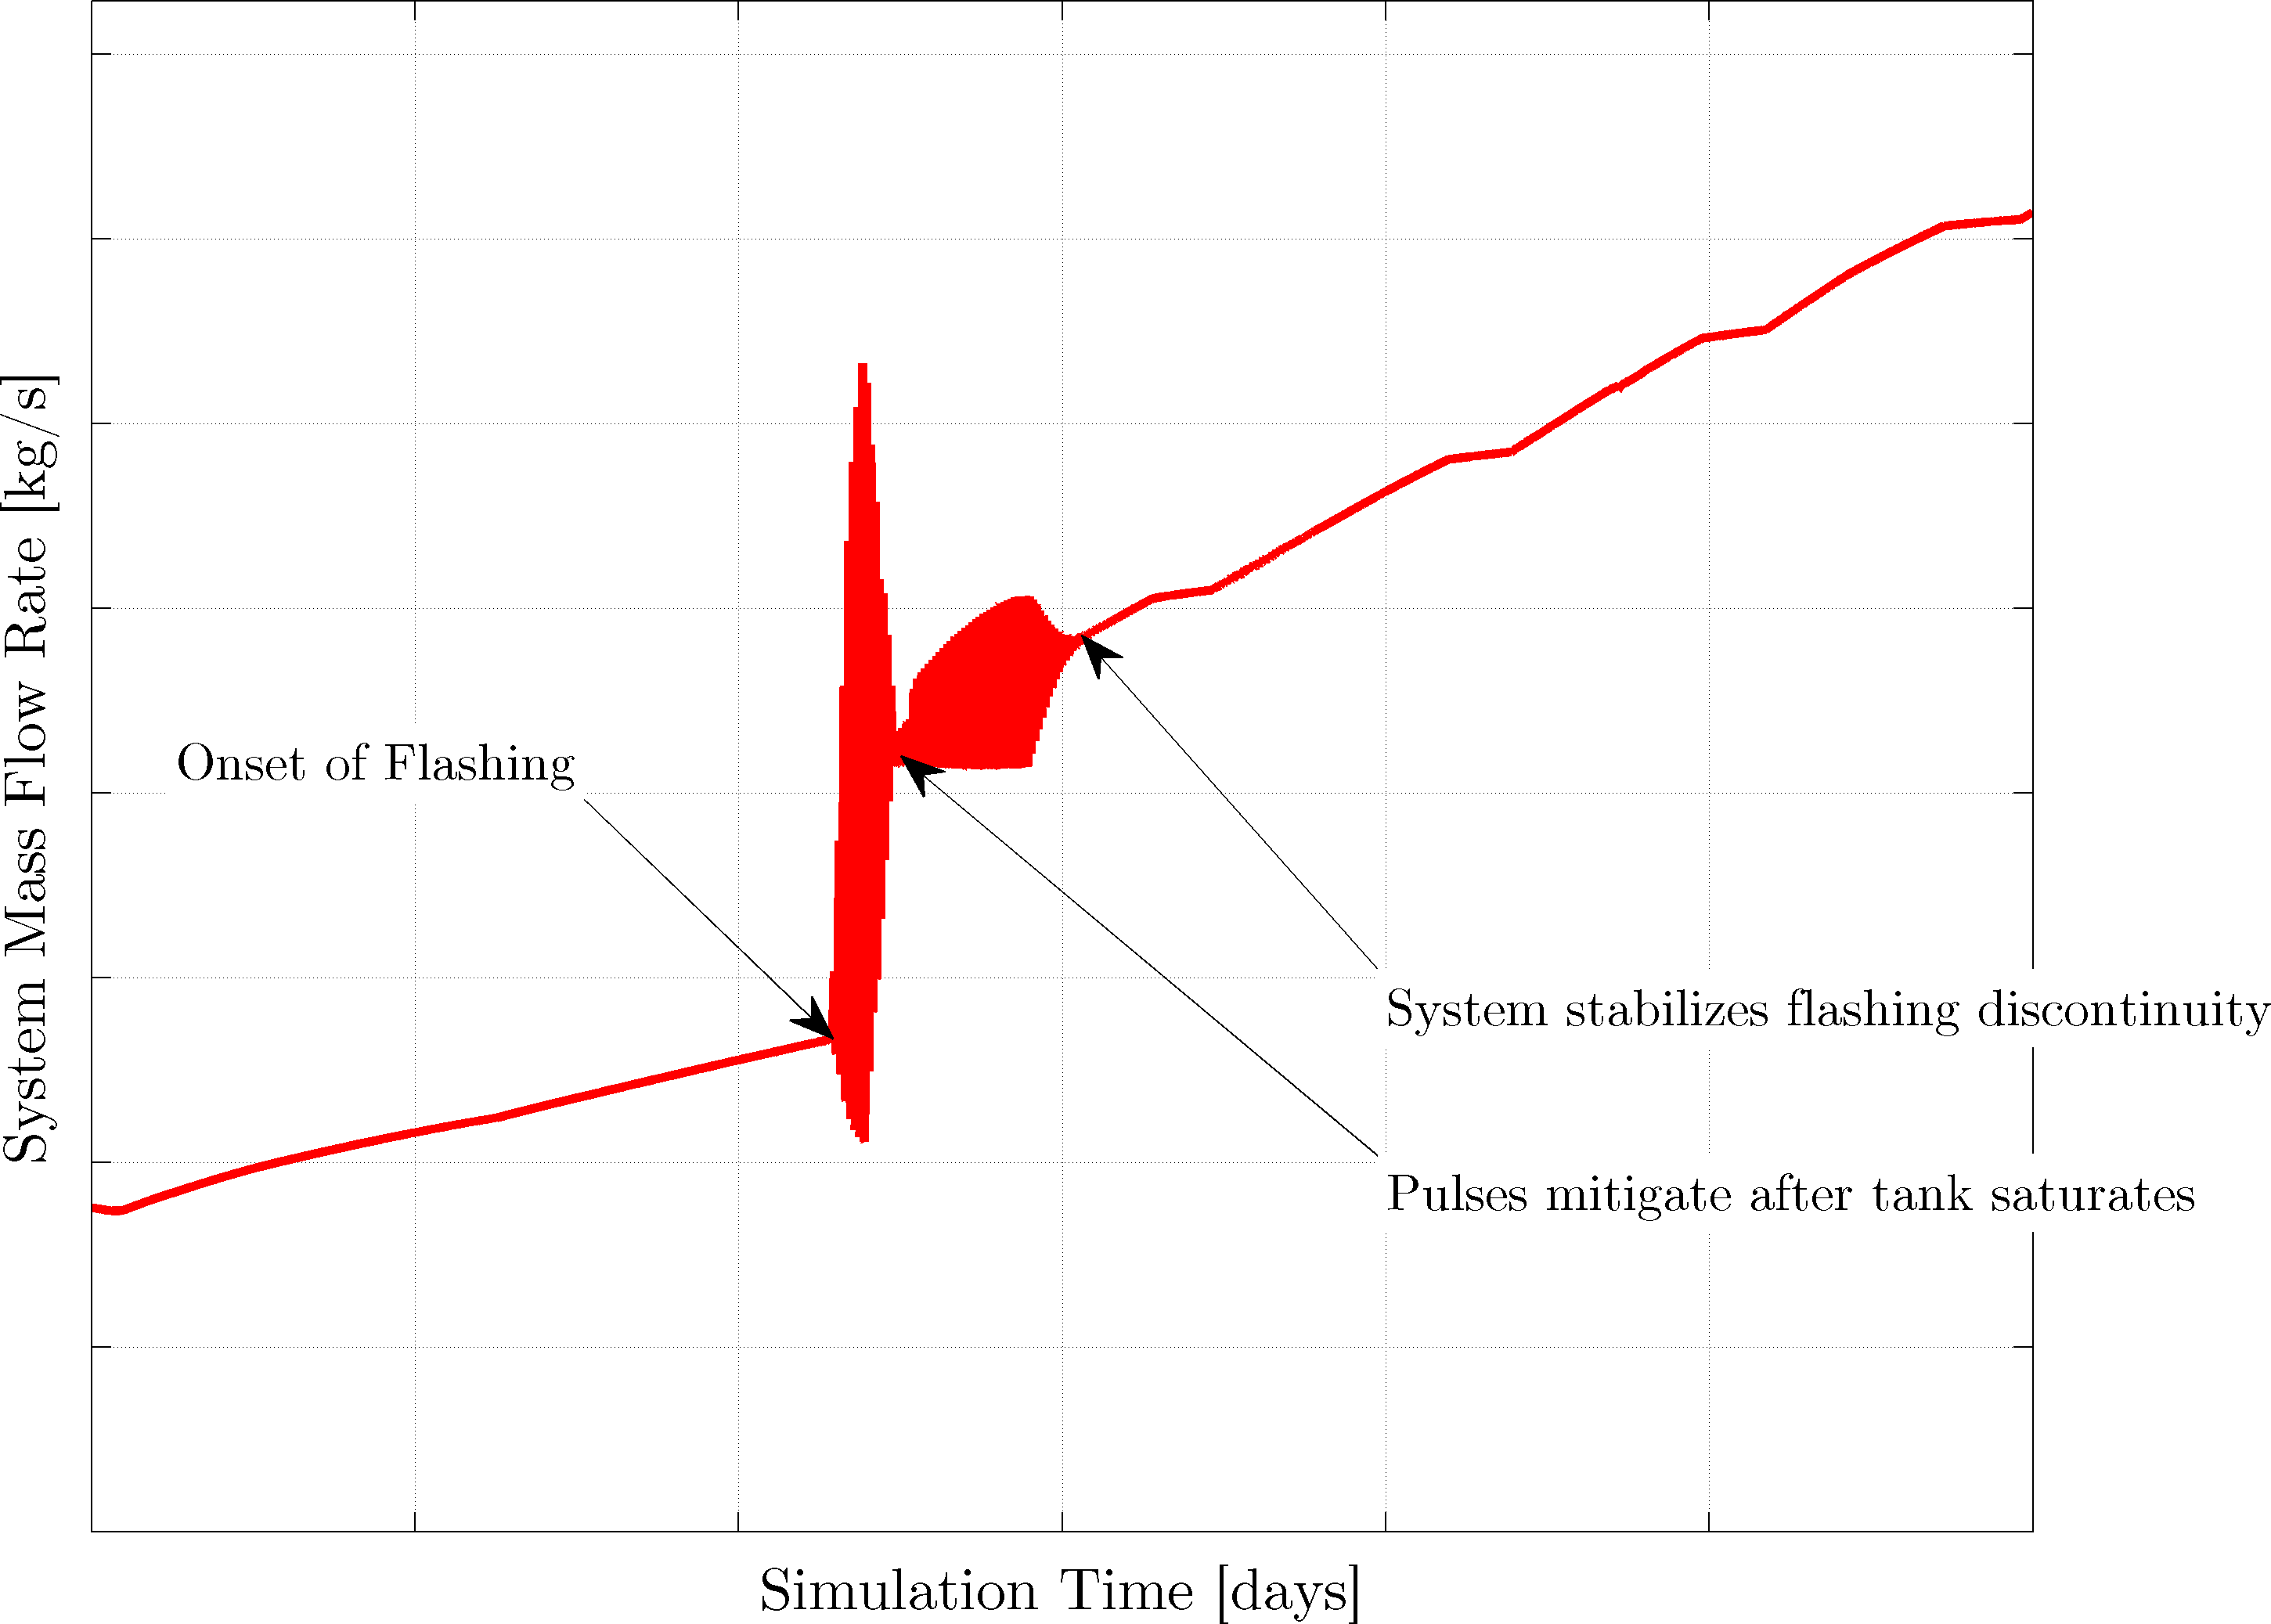
\includegraphics[width=0.9\textwidth]{PowerProfiles_MassFlowRateAnnotationsThesis.png}%
\end{figure}

\subsection{\TheUniversity\ RCCS Experiment}
Since the \Acronym{RCCS} discussed above exists purely on paper, an experiment was built at the \TheUniversity\ to directly observe and measure the behavior of an \Acronym{RCCS}-like system.
The experiment, presented in-brief by \cref{Figure:RCCSExperimentOverview}, is a scaled version of the full-scale \Acronym{RCCS} in terms of both dimension and number of risers.
While the full-scale system spans tens of meters with hundred of tubes, the experiment was scaled to a total height of approximately seven meters with three riser tubes.
Heaters mounted opposite the riser tubes provide the power to drive the natural circulation of the system.

\begin{figure}%
    \centering
    \caption[RCCS Experiment Full System diagram]{An overview of the whole RCCS experiment with important sections annotated.}%
    \label{Figure:RCCSExperimentOverview}%
    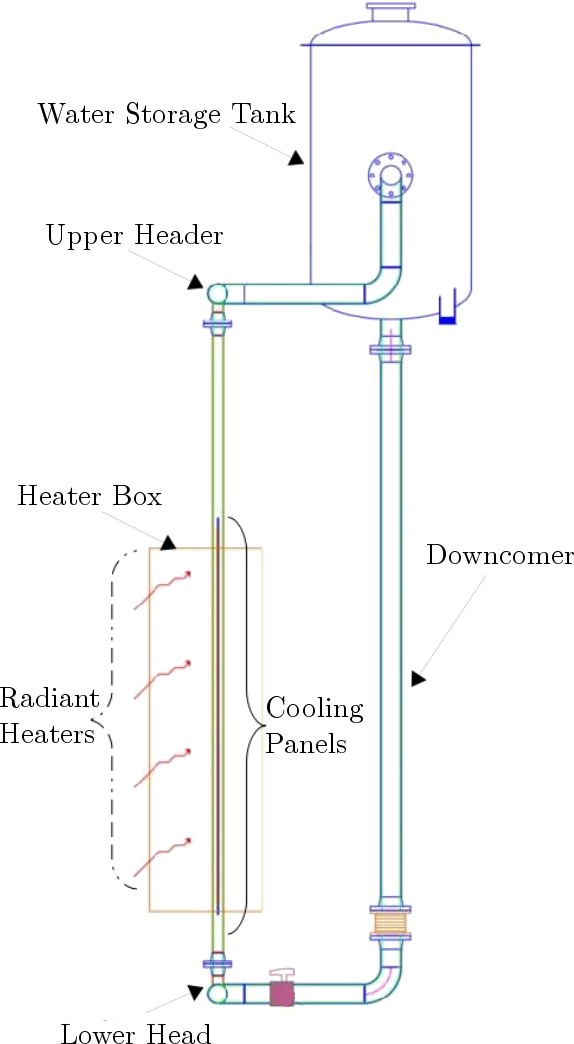
\includegraphics[height=0.50\textheight]{RCCSExperimentOverview.png}
    \vspace*{4em}
%\end{figure}%
%\begin{figure}%
    \centering
    \caption[RCCS Experiment Three Riser diagram]{An overview of the RCCS experiment's three riser/radiant heater setup.}%
    \label{Figure:RCCSExperimentHeatBox}%
    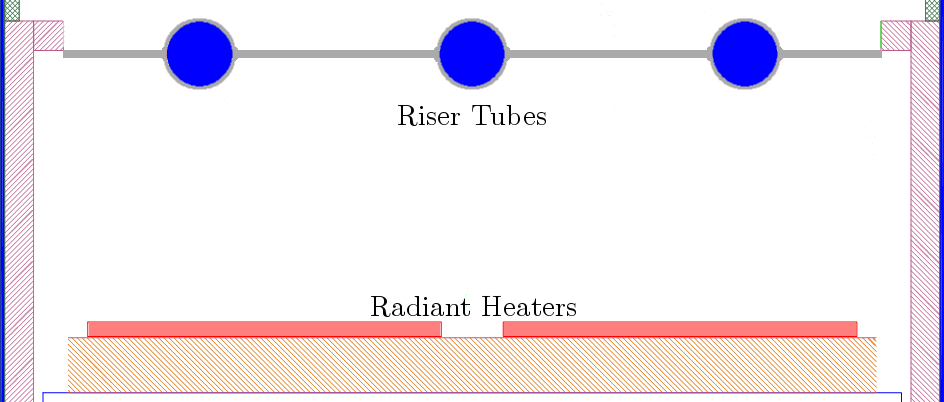
\includegraphics[width=0.80\textwidth]{RCCSExperimentHeatBox.png}%
\end{figure}

Due to the smaller scale and detailed design, a more precise numerical model could be made and benchmarked against data.
The full convection/radiation enclosure for the heater box was used to simulate station blackout conditions as in the full-scale with a scaled heat flux.
The mass flow rates from each of the risers for this accident simulation are shown in \cref{Figure:ExperimentMassFlowRateVsTime}.
The highly oscillatory nature of the flow rate after flashing begins is not only present but metastasized in this experiment.
Additionally, reverse flows in two of the risers is present (though the total system mass flow rate is always positive).
This local reversal of flow is more than likely systemic since short piping at the top allows a two-phase condition to exist at the top of the red riser.
While not expected in the full-scale system, this flow reversal is an interesting feature of the experiment's design and should be investigated.

\begin{figure}%
    \centering
    \begin{subfigure}[t]{\textwidth}
        \centering  
        \caption[ Mass flow rate versus time for the three riser tubes]{   
            Mass flow rate versus time for the three riser tubes of the RCCS experiment with station blackout accident conditions. 
            The colors of the plot lines correspond to the riser colors in \cref{Figure:RCCSExperimentRiserPlotAid}.}%
        \label{Figure:ExperimentMassFlowRateVsTime}%
        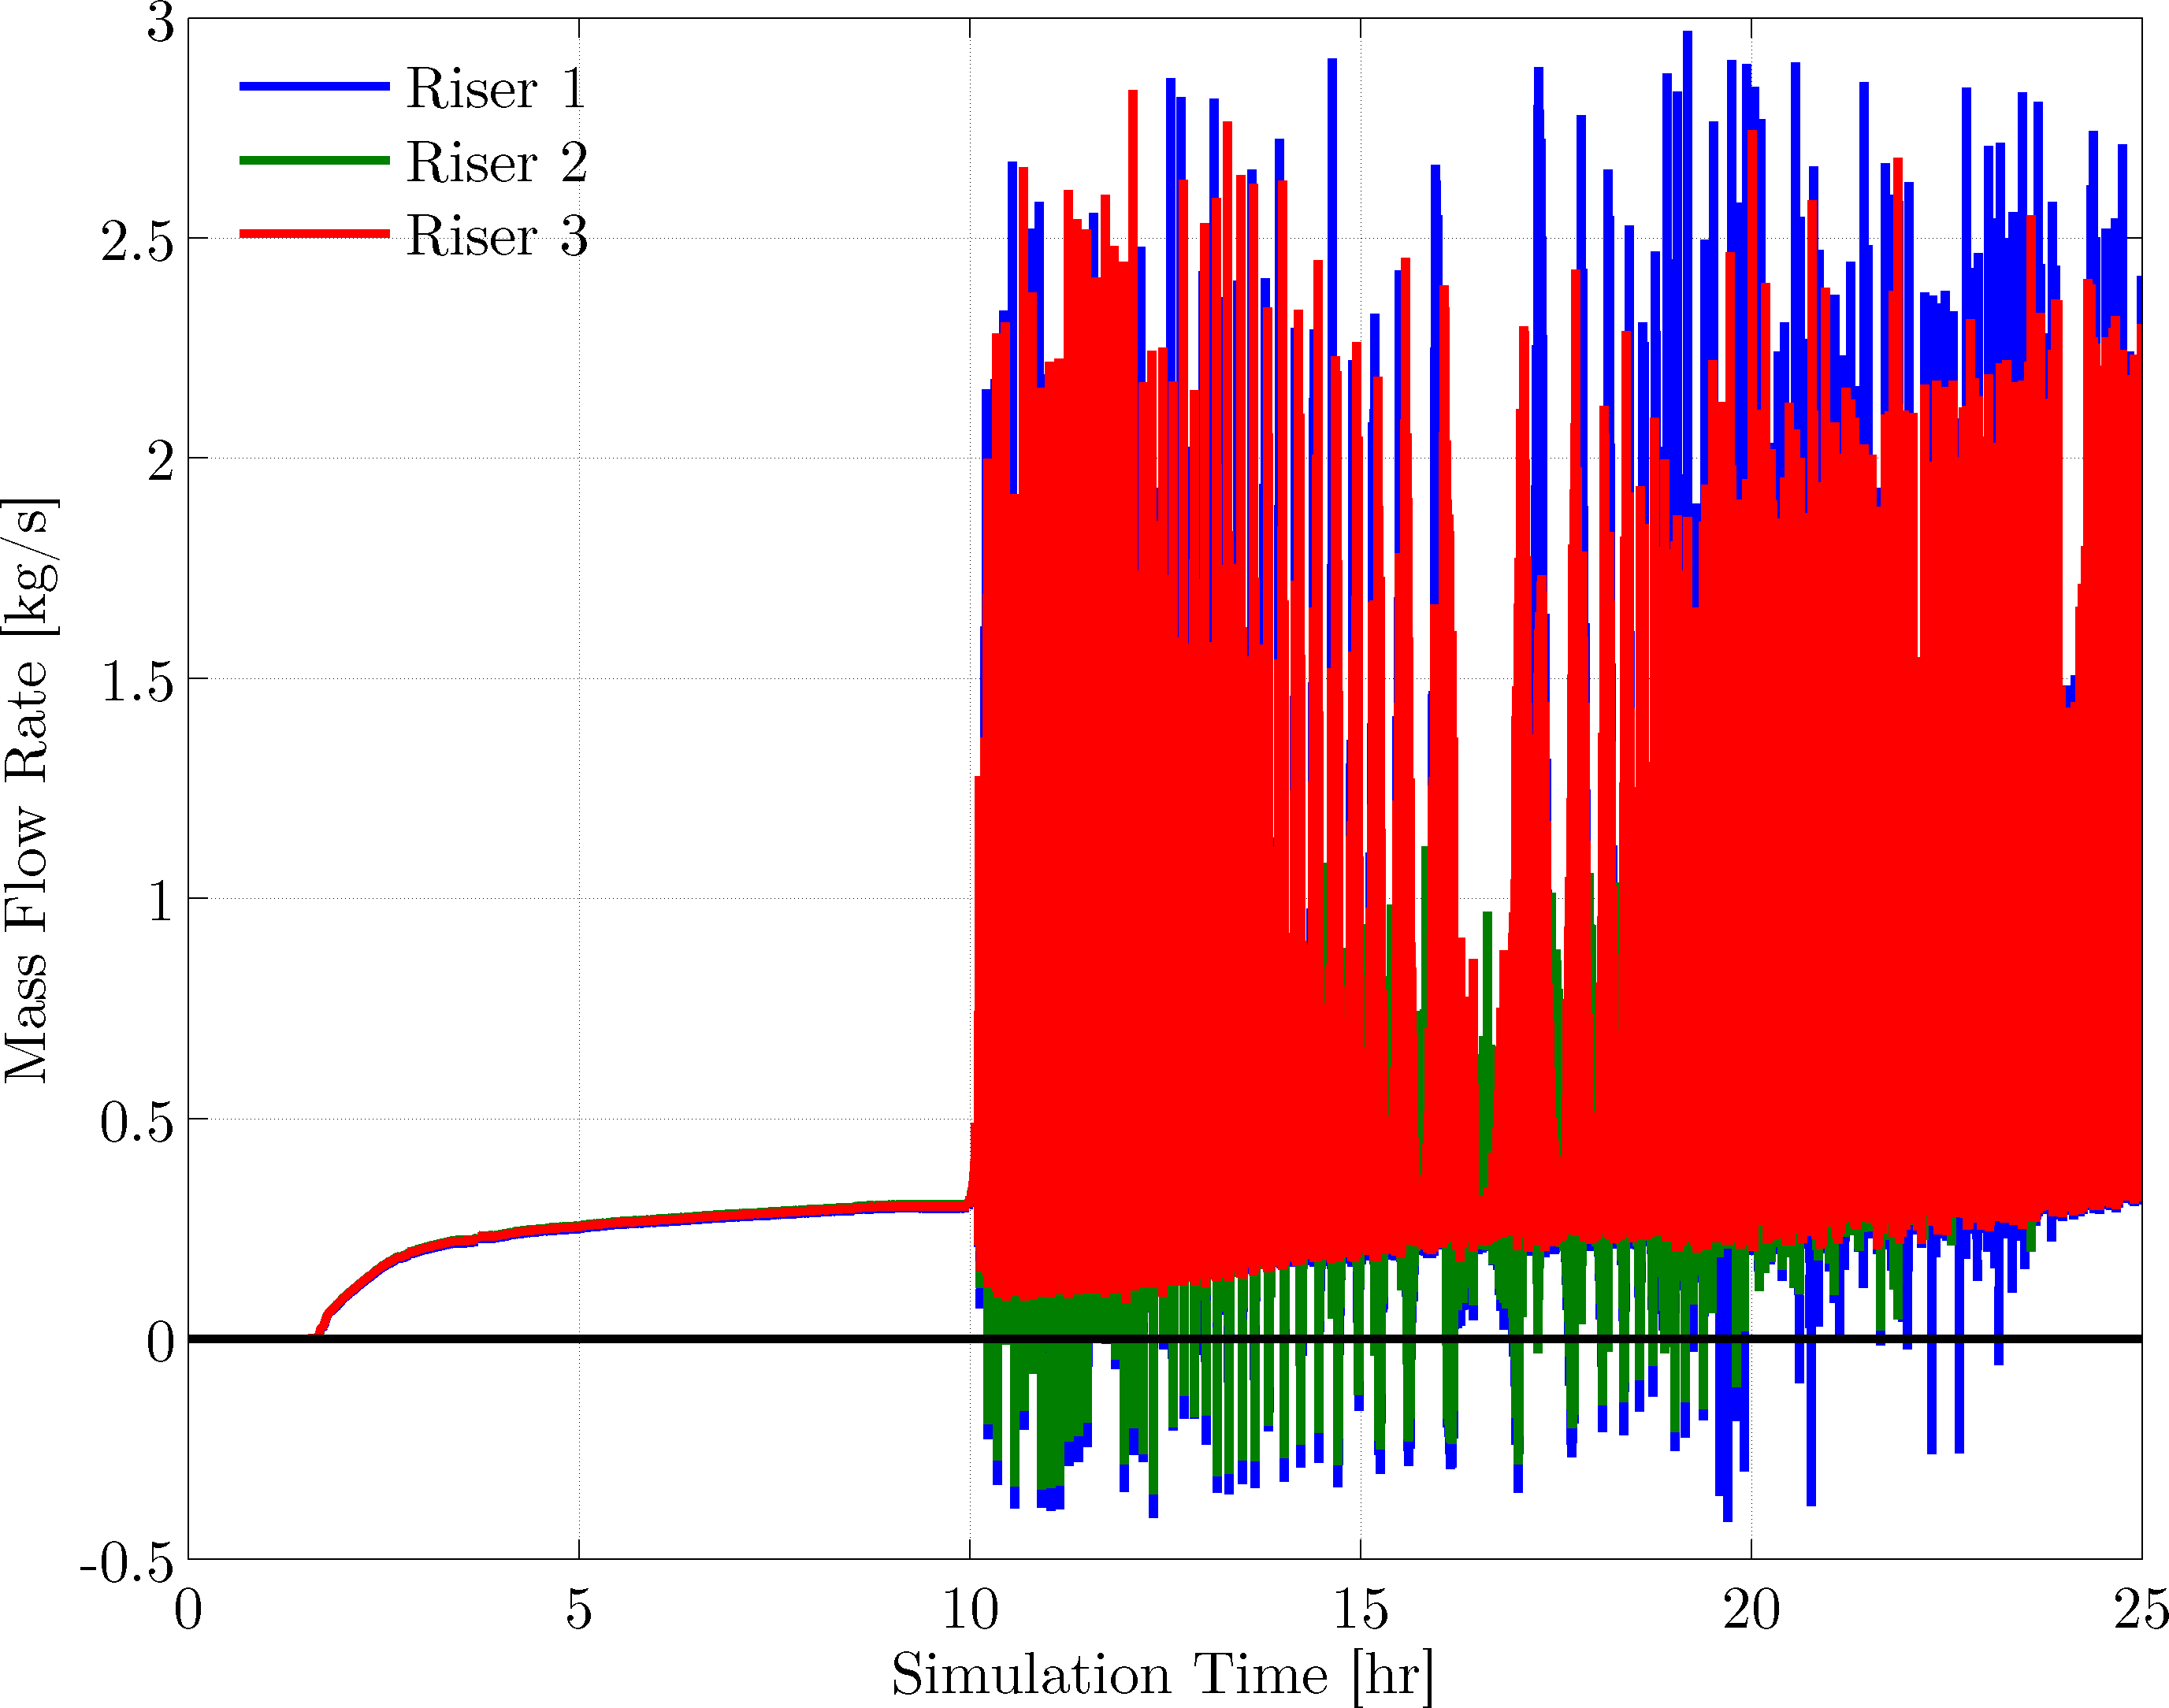
\includegraphics[width=0.75\textwidth]{ExperimentMassFlowRateVsTime.png}
    \end{subfigure}
    \vskip3em
    \begin{subfigure}[t]{\textwidth}
        \centering
        \caption[Basic layout of the RCCS experiment]{Basic layout of the RCCS experiment's numerical model.
                 The blue and red outlines denote the cooling and heating zones, respectively.}%
        \label{Figure:RCCSExperimentRiserPlotAid}%
        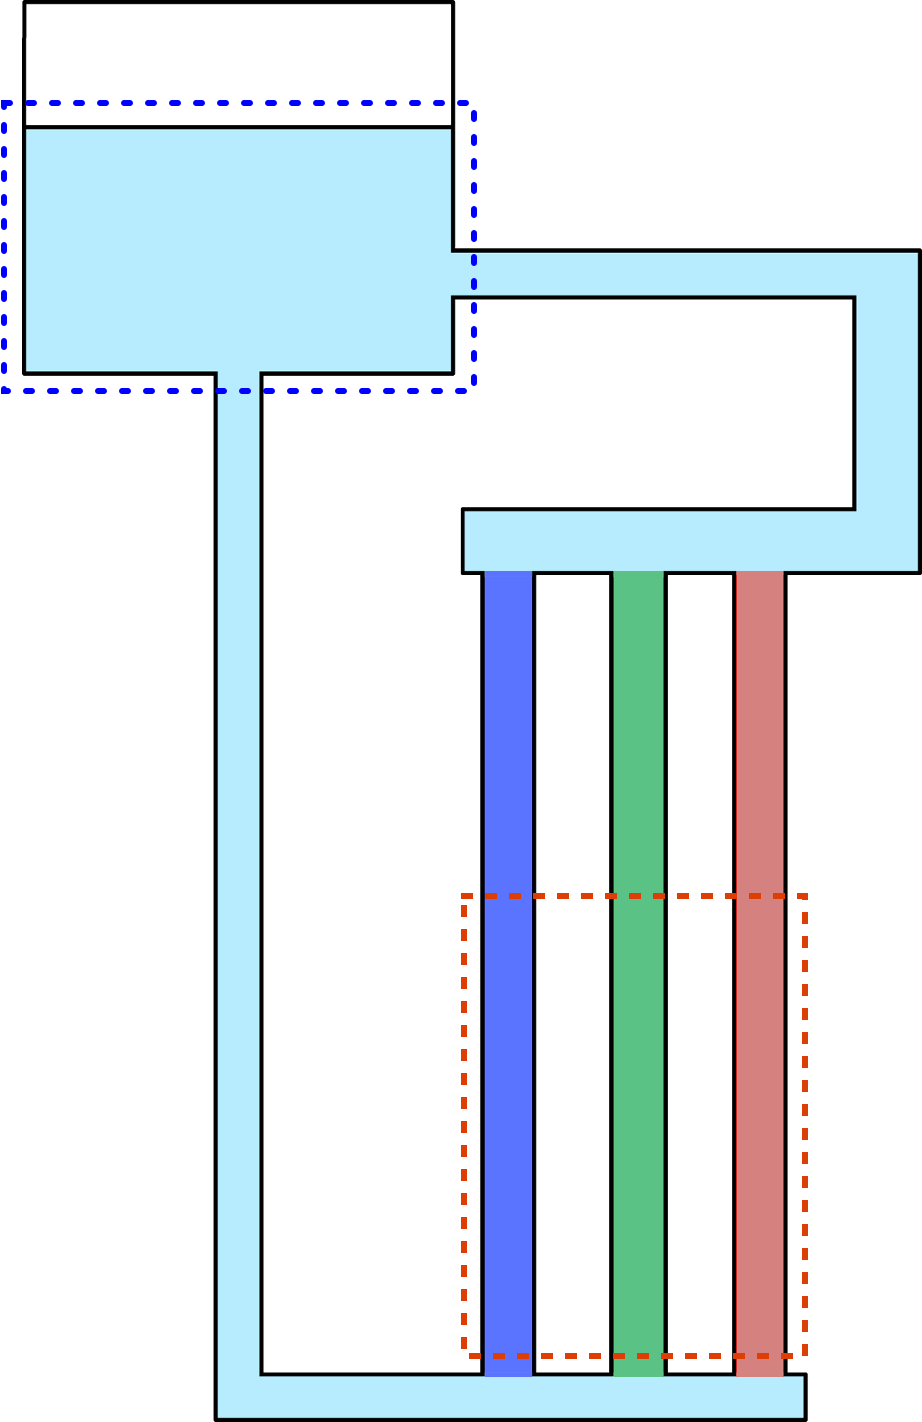
\includegraphics[height=0.35\textheight]{RCCSExperimentRiserPlotAid.png}%
    \end{subfigure}
\end{figure}
